REST is the software architecture style\cite{REST-wiki}. The communication is usually carried through HTTP protocol, but this is not a requirement. REST systems expose interfaces via URIs like\label{example-URI} \verb|/user| and then to interact with this resource one can use standard HTTP verbs (GET, POST, PUT and so on), but it does not need to implement all of them. Every new attempt to interact with resources is stateless, but there is a possibility of carrying additional information (i.e.\ for authorization) through HTTP headers.

\section{Explanation of architecture}
Architecture contains main server which serves data to clients (in this case users equipped with web browsers). Then it communicate with backend servers through RESTful API to get data for clients.

In addition main server is an entity which can represent multiple servers hidden behind load balancer for scaling for high load plus one additional server for storing database and shared files via NFS\@.

\begin{figure}[!htbp]
\centering
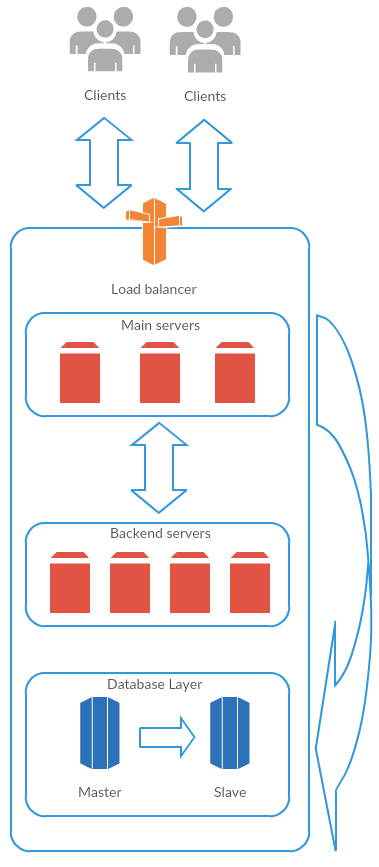
\includegraphics[scale=0.5]{architecture}
\label{fig:architecture}
\caption{Architecture of the whole system}
\end{figure}


\section{Principles}
REST is a set of principles that one can, but does not have fulfill. If criteria are met it can be said that implemented architecture is RESTful. Following sections present necessary principles that needs to be achieved.

\subsection{Uniform interface}
\label{uniform-interface}
In case of HTTP form of transporting data, every interaction can be made only through defined set of HTTP verbs as follows:

\begin{table}[!htbp]
\centering
\begin{tabular}{ll} \toprule
 HTTP verb &  Meaning \\ \midrule
 GET & Fetch resource \\
 POST & Create new resource \\
 PUT & Update resource by replacing \\
 PATCH & Update resource partially \\
 DELETE & Remove resource \\
 OPTIONS & Get list of available HTTP verbs \\ \bottomrule
\end{tabular}
\caption{HTTP verbs}
\label{tab:http-verbs}
\end{table}

Basically, in case of our example resource \verb|/user| GET, POST, PUT, PATCH, DELETE, OPTIONS would mean get user data, create new user, modify user by replacing all his data, update only few things (i.e.\ email and password), remove user, get available options (to see if I can remove user or not) respectively.

\subsection{Stateless}
\label{sec:stateless}
It means no single request depends on the previous one. By that less complexity is achieved, but as a drawback it should carry authorization information with each request (i.e.\ in HTTP headers) causing more bandwidth usage.

\subsection{Resources exposed via URIs}
\label{sec:resources}
URI\cite{URI-wiki} in short, it is a sequence of digits called string that represents specific resource. It is used commonly in WWW\@. A good example will be
\begin{verbatim}
http://google.com/a
\end{verbatim}
Breaking this up it begins with protocol name. In this case \verb|http|. Then it follows the domain name (\verb|google.com|). Those two are called URL and then after a last slash we have \verb|a| which is called URN\@. REST also tells that the URIs should be elegant, descriptive and not confusing so their meanings is straightforward.

\section{Framework design}
For the purpose of implementing aforementioned architecture a framework was created in new language ``Go'' backed by Google\cite{Go-wiki}. It can be further reused in other projects as it was released as a Free Software. The choice of Go as a language is not accidental. It has a really well defined standard library and it is very secure statically typed language with no implicit types conversions. Not to mentioned that is really fast in execution, but as a drawback writing a code feels really verbose.

Framework uses middlewares for modifying every new request and then response that is sent to a user. For instance we can create middleware purely for authentication process. If the user malformed credentials then middleware will modify the response so that the user knows that he provided them wrong.

\begin{figure}[!htbp]
\centering
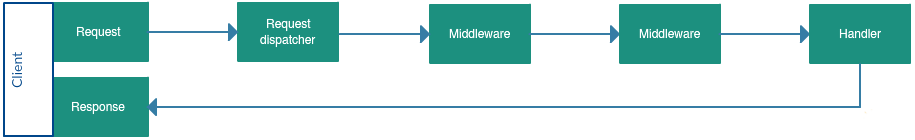
\includegraphics[scale=0.45]{middleware}
\caption[Request flow through middlewares]{Request flow through middlewares. Note that each middleware can modify request and response as they wish.}
\label{fig:middleware}
\end{figure}

\section{Authentication system and security}
Authentication system is implemented as middleware and uses standardized JWT tokens\cite{JWT-rfc}. The big benefit is that we do not need to store session in our database, we only need to verify that the token was signed by us.

The security is implemented at different levels. Connection is secured by standard TLS/SSL on HTTP level. Some resources require user to be authenticated (valid token).


\section{Strengths and weaknesses}
REST services are created from well known defined standards such as XML, JSON, URI, HTTP\@. They provide simple interfaces and they are simple to use in general. All web browsers are supporting aforementioned standards and most big websites chosen to implement RESTful services.

By it stateless nature it proves to scale well for many clients and removes complexity which has a big impact on performance and reliability.

When REST is using HTTP as a communication layer it can leverage the benefits of this protocol by using caching, clustering and load balancing which is a big win for architectures that needs to scale for millions of users.

REST was defined in 2000\cite{REST-wiki} as a style and design architecture, but being heavily tightened to HTTP it inherited all its limitations like GET can only carry 4~KB of input data\cite[p.~3]{restful-web-services}.

Another thing is performance when sending big amount of data and initializing connection every time we want to interact with resources. Unlike WebSockets, in REST we must send all the headers every time we communicate. In real time applications it is a big issue\footnote{That is the main reason behind creation of WebSockets}.

Last weakness is lack of defined security and authentication methods in standard. Therefore developers have to use TLS/SSL to secure communication and create authentication system by themselves.
